	\subsubsection*{Informazioni sul package}
		\begin{figure}[h]
			\centering
			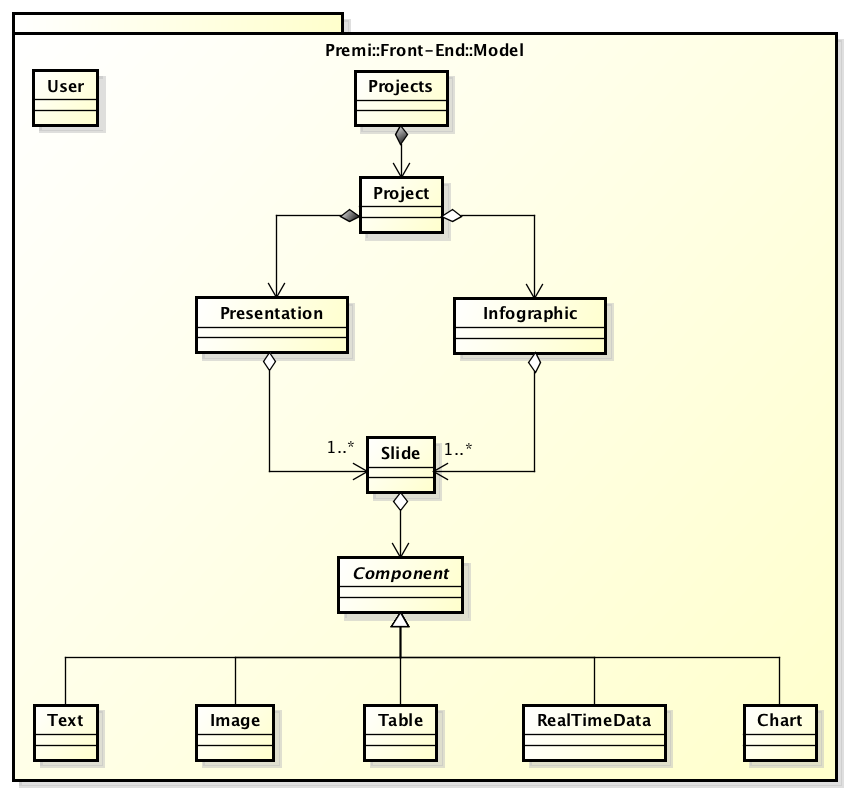
\includegraphics[width=0.9\linewidth]{img/front-end_model}
			\caption[Premi::Front-End::Model]{Premi::Front-End::Model}
		\end{figure}
		Il package serve per mantenere i dati relativi al \textit{front-end} e tutta la loro logica di business.

	\subsubsection*{Classi contenute}
		\begin{itemize}
		 \item Premi::Front-End::Model::Projects:
			\begin{itemize}
				\item \textbf{Descrizione}:classe per la gestione di una collezione di progetti.Un progetto racchiude una presentazione e zero o più infografiche.
				\item \textbf{Relazioni con altre classi}:
				\begin{itemize}
					\item Premi::Front-End::Model::Project.
				\end{itemize}
			\end{itemize}
		\item  Premi::Front-End::Model::Project: 
			 \begin{itemize}
				\item \textbf{Descrizione}: classe per la gestione di un progetto.
				\item \textbf{Relazioni con altre classi}:
				\begin{itemize}
					\item Premi::Front-End::Model::Presentation.
					\item Premi::Front-End::Model::Infographic.
				\end{itemize}
			\end{itemize}
		 \item  Premi::Front-End::Model::Infographic:
			\begin{itemize}
				\item \textbf{Descrizione}: classe per la gestione di una infografica. Un'infografica ha il compito di raggruppare piu slide in un template grafico scelto dall'utente in un ordine impostabile di volta in volta.
				\item \textbf{Relazioni con altre classi}:
				\begin{itemize}
					\item Premi::Front-End::Model::Slide.
				\end{itemize}
			\end{itemize}
		 \item   Premi::Front-End::Model::Presentation:
			\begin{itemize}
				\item \textbf{Descrizione}: classe per la gestione di una presentazione. Una presentazione raggruppa più slide. Per la visualizzazione delle presentazioni è stato scelto di utilizzare il framework Reveal.js che permette di avere una visualizzazione a griglia, di conseguenza una presentazione deve memorizzare anche le coordinate delle sue slide.
				\item \textbf{Relazioni con altre classi}:
				\begin{itemize}
					\item Premi::Front-End::Model::Slide.
				\end{itemize}
			\end{itemize}
		 \item Premi::Front-End::Model::Slide: Classe per la gestione di una slide.
			\begin{itemize}
				\item \textbf{Descrizione}: classe per la gestione di una slide.
				\item \textbf{Relazioni con altre classi}:
				\begin{itemize}
					\item Premi::Front-End::Model::Component.
				\end{itemize}
			\end{itemize}
		 \item  Premi::Front-End::Model::Component: 
			\begin{itemize}
				\item \textbf{Descrizione}: Classe astratta concretizzata ed estesa dalle varie componenti implementando il pattern \textit{composite} per fare si che elementi foglia e collezione vengano trattati allo stesso modo. Nello specifico, una tabella rappresenta un aggregato di altre componenti.
			\end{itemize}
		 \item  Premi::Front-End::Model::Text:
			\begin{itemize}
				\item \textbf{Descrizione}: classe per la gestione di un elemento testuale e delle sue proprietà di formattazione. Concretizza ed estende Premi::Front-End::Model::Component.
				\item \textbf{Relazioni con altre classi}:
				\begin{itemize}
					\item Premi::Front-End::Model::Component.
				\end{itemize}
			\end{itemize}
		 \item  Premi::Front-End::Model::Image:
			\begin{itemize}
				\item \textbf{Descrizione}: lasse per la gestione di un elemento di tipo immagine.
				\item \textbf{Relazioni con altre classi}:
				\begin{itemize}
					\item Premi::Front-End::Model::Component.
				\end{itemize}
			 \end{itemize}
		 \item  Premi::Front-End::Model::Table:
			\begin{itemize}
				\item \textbf{Descrizione}: classe per la gestione di una tabella. Una tabella può contenere altre componenti che concretizzano la classe Premi::Front-End::Model::Component.
				\item \textbf{Relazioni con altre classi}:
				\begin{itemize}
					\item Premi::Front-End::Model::Component.
				\end{itemize}
			 \end{itemize}
		 \item  Premi::Front-End::Model::RealTimeData:
			\begin{itemize}
				\item \textbf{Descrizione}: classe per la gestione di componenti che si aggiornano in tempo reale con cadenza personalizzabile.
				\item \textbf{Relazioni con altre classi}:
				\begin{itemize}
					\item Premi::Front-End::Model::Component.
				\end{itemize}
			 \end{itemize}
		 \item  Premi::Front-End::Model::Chart: 
			\begin{itemize}
				\item \textbf{Descrizione}: classe per la gestione dei dati necessari per disegnare un grafico.
				\item \textbf{Relazioni con altre classi}:
				\begin{itemize}
					\item Premi::Front-End::Model::Component.
				\end{itemize}
			 \end{itemize}
		 \item  Premi::Front-End::Model::User:
			\begin{itemize}
				\item \textbf{Descrizione}: classe per la gestione degli utenti.
			 \end{itemize}

		 \end{itemize}